\documentclass[tikz,border=3pt]{standalone}
\usepackage{amsmath,amssymb}
\usetikzlibrary{arrows.meta,calc}
\definecolor{curveblue}{HTML}{245C86}
\definecolor{accent}{HTML}{A65E2E}
\definecolor{curveteal}{HTML}{287B6D}
\definecolor{curveviolet}{HTML}{76578B}
\begin{document}
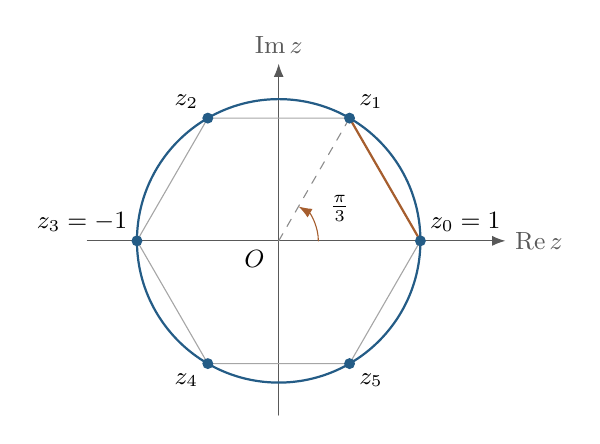
\begin{tikzpicture}[font=\small,>=Latex,line cap=round,line join=round]
\begin{scope}[scale=1.8]
\draw[->,black!65] (-1.350000,0.000000)--(1.600000,0.000000) node[right]{$\operatorname{Re}z$};
\draw[->,black!65] (0.000000,-1.230000)--(0.000000,1.250000) node[above]{$\operatorname{Im}z$};
\draw[curveblue,thick] (0,0) circle (1);
\draw[black!35] (1.000000,0.000000)--(0.500000,0.866025)--(-0.500000,0.866025)--(-1.000000,0.000000)--(-0.500000,-0.866025)--(0.500000,-0.866025)--cycle;
\draw[accent,thick] (1,0)--(.5,.866025);\draw[black!45,dashed] (0,0)--(.5,.866025);
\draw[accent,->] (.28,0) arc[start angle=0,end angle=60,radius=.28];\node at (.43,.23) {$\frac\pi3$};
\fill[curveblue] (1.000000,0.000000) circle (1.1pt);
\node[above right] at (1.000000,0.000000) {$z_0=1$};
\fill[curveblue] (0.500000,0.866025) circle (1.1pt);
\node[above right] at (0.500000,0.866025) {$z_1$};
\fill[curveblue] (-0.500000,0.866025) circle (1.1pt);
\node[above left] at (-0.500000,0.866025) {$z_2$};
\fill[curveblue] (-1.000000,0.000000) circle (1.1pt);
\node[above left] at (-1.000000,0.000000) {$z_3=-1$};
\fill[curveblue] (-0.500000,-0.866025) circle (1.1pt);
\node[below left] at (-0.500000,-0.866025) {$z_4$};
\fill[curveblue] (0.500000,-0.866025) circle (1.1pt);
\node[below right] at (0.500000,-0.866025) {$z_5$};
\node[below left] at (-0.030000,0.000000) {$O$};
\end{scope}
\end{tikzpicture}
\end{document}
